%!TEX root = ../paper.tex
\section{Video Classification in Caffe}
\label{sec:classification}

...\todo{general introduction}

The architecture of our artificial neural network was build on the work of ...\todo{reference}.
It is a three-stream architecture (Figure~\ref{fig:architecture}).
The first stream is processing the single frames of a video, further called \emph{spatial}.
This stream is responsible for recognizing objects in frames.
The second stream memorizes motion of certain actions.
This stream handles flow images and is therefore called \emph{flow}.
Both streams consists of a convolutional neural network (CNN) followed by a LSTM.
To merge the predictions of both streams a third stream is introduced by ...\todo{reference}.
This stream, called \emph{fusion}, takes the output of the CNN and merge the predictions.
The output of all three streams is then combined in the end to get a final prediction.
\begin{figure}[!htb]
	\centering
	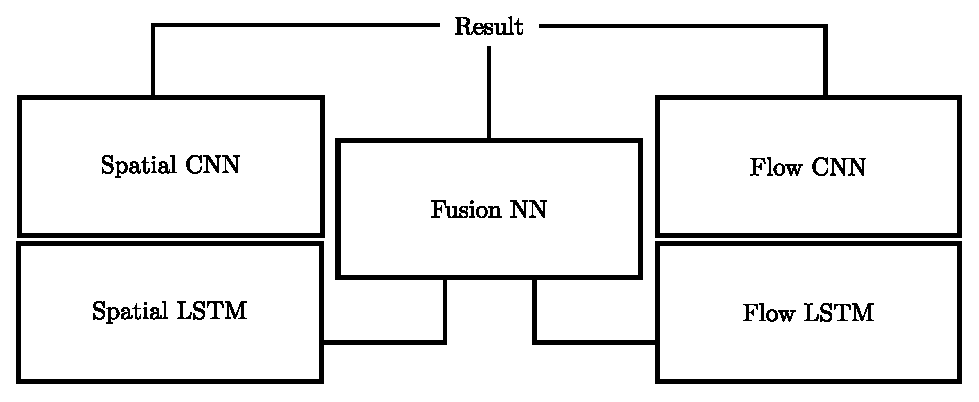
\includegraphics[scale=.7]{images/architecture.eps}
	\caption{General Architecture TODO}
	\label{fig:architecture}
\end{figure}

The individual neural networks used in this architecture differ from the work of ...\todo{reference}.
During our research we tried out different neural networks for the two streams, which will be presented in this section.
Also the parameters, which were used for the training, and the results will be shown.

\subsection{Changes to Caffe-tmbo}

\begin{itemize}
	\item New sequence data layer
	\item Multi-layer script
	\item More?
\end{itemize}

\subsection{Spatial}
\label{subsec:spatial}

\begin{itemize}
	\item
		Different nets:
		\begin{itemize}
			\item Caffenet/CNN\_M (also tried, VGG 19, but too big)
			\item With weights/without weights
			\item Compare the nets with respect to memory, number of parameters, training time, performance
		\end{itemize}
	\item
		Experiments:
		\begin{itemize}
			\item Different dropouts
			\item Train from scratch vs train from weights
			\item On different splits?
			\item Fc6, Fc7, fc8
			\item Different base data sets (only 16, all data)
			\item Different flows?
			\item Occlusion tests
		\end{itemize}
	\item
		LSTM did not work out
\end{itemize}


\subsection{Flow}
\label{subsec:flow}


\subsection{Fusion}
\label{subsec:fusion}
As first approach we rebuild the fusion architecture presented by TODO.

We took the CNN nets for spatial and flow presented above and build a fusion architecture on top of them.
Both CNNs were cut off after the \textit{fc6}-layer having an output of 16 x 4096.\todo{Der eigentlich output von fc6 ist ja erstmal 1 x 4096}
The input to the CNNs were 16 frames per video.
So the output of the \textit{fc6}-layer of the spatial and flow net correspond to a prediction for each of those frames.
To fuse those predictions, the first step is to merge the 16 prediction of one video into one prediction for the whole video.
Therefore, we take the average prediction for both spatial and flow.
A fully-connected layer is then trained with those predictions before we concatenate the predictions of spatial and flow.
In the end two fully-connected layer are trained on the merged predictions.
The output is defined by an accuracy layer.
The whole architecture is shown in Figure~\ref{fig:fusion_architecture}\todo{improve figure}.
\begin{figure}[!htb]
	\centering
	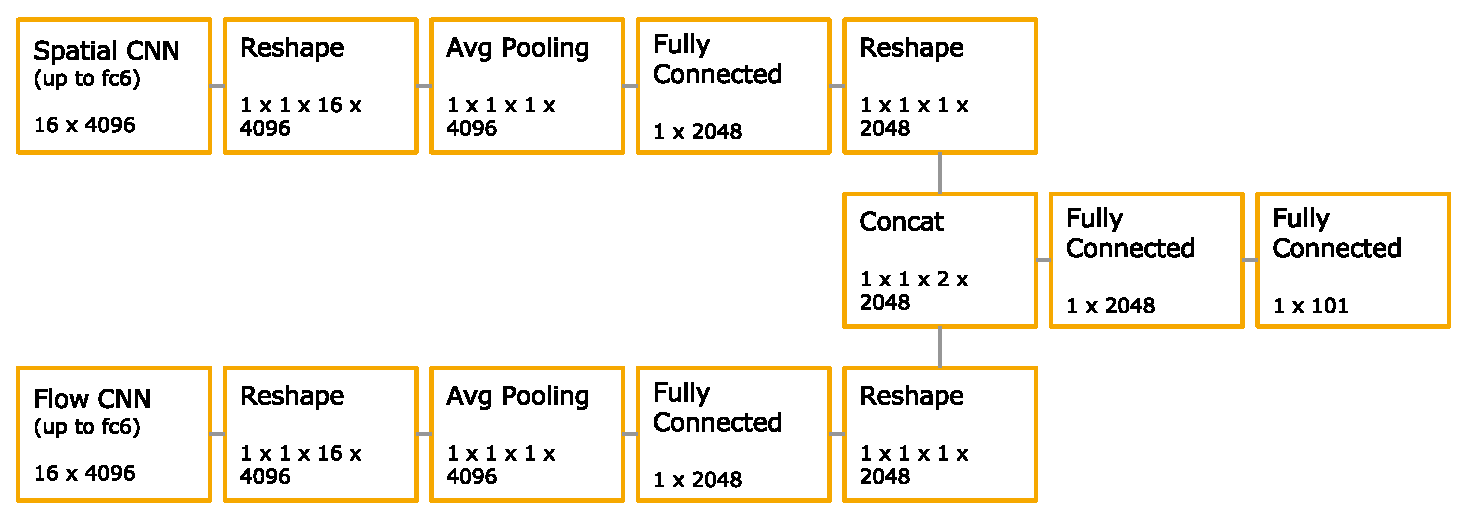
\includegraphics[scale=.7]{images/fusion_architecture.eps}
	\caption{Architecture of the fusion net: The predictions per frame of one video from the spatial and flow net are merged into one prediction per video each. Those predictions are then merged and trained via two fully connected layers.}
	\label{fig:fusion_architecture}
\end{figure}






